% Created by tikzDevice version 0.12.3.1 on 2022-05-26 15:31:38
% !TEX encoding = UTF-8 Unicode
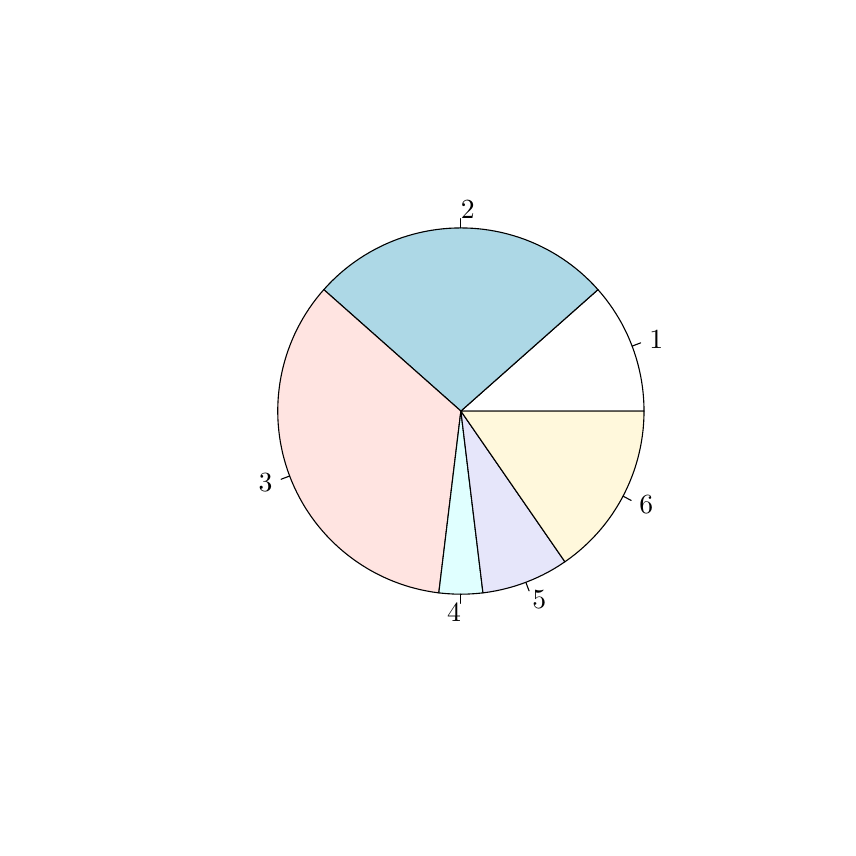
\begin{tikzpicture}[x=1pt,y=1pt]
\definecolor{fillColor}{RGB}{255,255,255}
\path[use as bounding box,fill=fillColor,fill opacity=0.00] (0,0) rectangle (289.08,289.08);
\begin{scope}
\path[clip] ( 49.20, 61.20) rectangle (263.88,239.88);
\definecolor{drawColor}{RGB}{0,0,0}
\definecolor{fillColor}{RGB}{255,255,255}

\path[draw=drawColor,line width= 0.4pt,line join=round,line cap=round,fill=fillColor] (222.72,150.54) --
	(222.68,152.72) --
	(222.57,154.90) --
	(222.39,157.07) --
	(222.14,159.24) --
	(221.82,161.39) --
	(221.43,163.54) --
	(220.96,165.67) --
	(220.43,167.79) --
	(219.83,169.88) --
	(219.16,171.96) --
	(218.42,174.01) --
	(217.61,176.03) --
	(216.74,178.03) --
	(215.80,180.00) --
	(214.80,181.94) --
	(213.73,183.84) --
	(212.60,185.70) --
	(211.41,187.53) --
	(210.16,189.32) --
	(208.86,191.07) --
	(207.49,192.77) --
	(206.07,194.42) --
	(156.54,150.54) --
	cycle;

\path[draw=drawColor,line width= 0.4pt,line join=round,line cap=round] (218.42,174.01) --
	(221.51,175.18);
\end{scope}
\begin{scope}
\path[clip] (  0.00,  0.00) rectangle (289.08,289.08);
\definecolor{drawColor}{RGB}{0,0,0}

\node[text=drawColor,anchor=base west,inner sep=0pt, outer sep=0pt, scale=  1.00] at (224.61,173.15) {1};
\end{scope}
\begin{scope}
\path[clip] ( 49.20, 61.20) rectangle (263.88,239.88);
\definecolor{drawColor}{RGB}{0,0,0}
\definecolor{fillColor}{RGB}{173,216,230}

\path[draw=drawColor,line width= 0.4pt,line join=round,line cap=round,fill=fillColor] (206.07,194.42) --
	(204.62,196.01) --
	(203.12,197.55) --
	(201.56,199.04) --
	(199.96,200.48) --
	(198.31,201.87) --
	(196.62,203.20) --
	(194.89,204.47) --
	(193.11,205.69) --
	(191.30,206.85) --
	(189.45,207.95) --
	(187.57,208.99) --
	(185.65,209.97) --
	(183.70,210.89) --
	(181.72,211.74) --
	(179.72,212.53) --
	(177.69,213.25) --
	(175.64,213.90) --
	(173.57,214.49) --
	(171.48,215.01) --
	(169.38,215.46) --
	(167.26,215.84) --
	(165.13,216.16) --
	(162.99,216.40) --
	(160.84,216.58) --
	(158.69,216.68) --
	(156.54,216.72) --
	(154.39,216.68) --
	(152.24,216.58) --
	(150.09,216.40) --
	(147.95,216.16) --
	(145.82,215.84) --
	(143.70,215.46) --
	(141.60,215.01) --
	(139.51,214.49) --
	(137.44,213.90) --
	(135.39,213.25) --
	(133.36,212.53) --
	(131.36,211.74) --
	(129.38,210.89) --
	(127.43,209.97) --
	(125.51,208.99) --
	(123.63,207.95) --
	(121.78,206.85) --
	(119.97,205.69) --
	(118.19,204.47) --
	(116.46,203.20) --
	(114.77,201.87) --
	(113.12,200.48) --
	(111.52,199.04) --
	(109.96,197.55) --
	(108.46,196.01) --
	(107.01,194.42) --
	(156.54,150.54) --
	cycle;

\path[draw=drawColor,line width= 0.4pt,line join=round,line cap=round] (156.54,216.72) --
	(156.54,220.03);
\end{scope}
\begin{scope}
\path[clip] (  0.00,  0.00) rectangle (289.08,289.08);
\definecolor{drawColor}{RGB}{0,0,0}

\node[text=drawColor,anchor=base west,inner sep=0pt, outer sep=0pt, scale=  1.00] at (156.54,220.13) {2};
\end{scope}
\begin{scope}
\path[clip] ( 49.20, 61.20) rectangle (263.88,239.88);
\definecolor{drawColor}{RGB}{0,0,0}
\definecolor{fillColor}{RGB}{255,228,225}

\path[draw=drawColor,line width= 0.4pt,line join=round,line cap=round,fill=fillColor] (107.01,194.42) --
	(105.63,192.82) --
	(104.30,191.17) --
	(103.03,189.48) --
	(101.81,187.75) --
	(100.65,185.98) --
	( 99.54,184.17) --
	( 98.50,182.33) --
	( 97.51,180.46) --
	( 96.58,178.56) --
	( 95.72,176.62) --
	( 94.92,174.67) --
	( 94.18,172.68) --
	( 93.50,170.68) --
	( 92.89,168.65) --
	( 92.34,166.61) --
	( 91.86,164.54) --
	( 91.45,162.47) --
	( 91.10,160.38) --
	( 90.82,158.28) --
	( 90.60,156.18) --
	( 90.46,154.07) --
	( 90.38,151.95) --
	( 90.37,149.83) --
	( 90.42,147.72) --
	( 90.55,145.61) --
	( 90.74,143.50) --
	( 91.00,141.40) --
	( 91.32,139.31) --
	( 91.72,137.23) --
	( 92.17,135.16) --
	( 92.70,133.11) --
	( 93.29,131.08) --
	( 93.94,129.06) --
	( 94.66,127.07) --
	( 95.44,125.11) --
	( 96.29,123.17) --
	( 97.20,121.25) --
	( 98.16,119.37) --
	( 99.19,117.52) --
	(100.27,115.70) --
	(101.42,113.92) --
	(102.62,112.18) --
	(103.87,110.47) --
	(105.18,108.81) --
	(106.54,107.19) --
	(107.95,105.61) --
	(109.41,104.08) --
	(110.92,102.60) --
	(112.48,101.16) --
	(114.08, 99.78) --
	(115.73, 98.45) --
	(117.41, 97.17) --
	(119.14, 95.94) --
	(120.91, 94.78) --
	(122.71, 93.66) --
	(124.54, 92.61) --
	(126.41, 91.62) --
	(128.31, 90.68) --
	(130.24, 89.81) --
	(132.20, 89.00) --
	(134.18, 88.26) --
	(136.18, 87.57) --
	(138.20, 86.95) --
	(140.25, 86.40) --
	(142.31, 85.91) --
	(144.38, 85.49) --
	(146.47, 85.13) --
	(148.56, 84.84) --
	(156.54,150.54) --
	cycle;

\path[draw=drawColor,line width= 0.4pt,line join=round,line cap=round] ( 94.66,127.07) --
	( 91.57,125.90);
\end{scope}
\begin{scope}
\path[clip] (  0.00,  0.00) rectangle (289.08,289.08);
\definecolor{drawColor}{RGB}{0,0,0}

\node[text=drawColor,anchor=base east,inner sep=0pt, outer sep=0pt, scale=  1.00] at ( 88.47,121.52) {3};
\end{scope}
\begin{scope}
\path[clip] ( 49.20, 61.20) rectangle (263.88,239.88);
\definecolor{drawColor}{RGB}{0,0,0}
\definecolor{fillColor}{RGB}{224,255,255}

\path[draw=drawColor,line width= 0.4pt,line join=round,line cap=round,fill=fillColor] (148.56, 84.84) --
	(151.21, 84.58) --
	(153.88, 84.42) --
	(156.54, 84.36) --
	(159.20, 84.42) --
	(161.87, 84.58) --
	(164.52, 84.84) --
	(156.54,150.54) --
	cycle;

\path[draw=drawColor,line width= 0.4pt,line join=round,line cap=round] (156.54, 84.36) --
	(156.54, 81.05);
\end{scope}
\begin{scope}
\path[clip] (  0.00,  0.00) rectangle (289.08,289.08);
\definecolor{drawColor}{RGB}{0,0,0}

\node[text=drawColor,anchor=base east,inner sep=0pt, outer sep=0pt, scale=  1.00] at (156.54, 74.54) {4};
\end{scope}
\begin{scope}
\path[clip] ( 49.20, 61.20) rectangle (263.88,239.88);
\definecolor{drawColor}{RGB}{0,0,0}
\definecolor{fillColor}{RGB}{230,230,250}

\path[draw=drawColor,line width= 0.4pt,line join=round,line cap=round,fill=fillColor] (164.52, 84.84) --
	(166.78, 85.16) --
	(169.03, 85.55) --
	(171.27, 86.02) --
	(173.48, 86.57) --
	(175.68, 87.19) --
	(177.86, 87.89) --
	(180.01, 88.66) --
	(182.13, 89.51) --
	(184.22, 90.43) --
	(186.28, 91.42) --
	(188.30, 92.48) --
	(190.29, 93.61) --
	(192.23, 94.81) --
	(194.13, 96.08) --
	(156.54,150.54) --
	cycle;

\path[draw=drawColor,line width= 0.4pt,line join=round,line cap=round] (180.01, 88.66) --
	(181.18, 85.57);
\end{scope}
\begin{scope}
\path[clip] (  0.00,  0.00) rectangle (289.08,289.08);
\definecolor{drawColor}{RGB}{0,0,0}

\node[text=drawColor,anchor=base west,inner sep=0pt, outer sep=0pt, scale=  1.00] at (182.35, 79.27) {5};
\end{scope}
\begin{scope}
\path[clip] ( 49.20, 61.20) rectangle (263.88,239.88);
\definecolor{drawColor}{RGB}{0,0,0}
\definecolor{fillColor}{RGB}{255,248,220}

\path[draw=drawColor,line width= 0.4pt,line join=round,line cap=round,fill=fillColor] (194.13, 96.08) --
	(195.93, 97.36) --
	(197.68, 98.70) --
	(199.38,100.10) --
	(201.04,101.56) --
	(202.65,103.07) --
	(204.20,104.63) --
	(205.71,106.24) --
	(207.16,107.91) --
	(208.55,109.62) --
	(209.88,111.37) --
	(211.16,113.17) --
	(212.37,115.02) --
	(213.53,116.90) --
	(214.62,118.81) --
	(215.64,120.77) --
	(216.60,122.75) --
	(217.49,124.77) --
	(218.32,126.82) --
	(219.08,128.89) --
	(219.76,130.98) --
	(220.38,133.10) --
	(220.92,135.24) --
	(221.40,137.39) --
	(221.80,139.56) --
	(222.13,141.74) --
	(222.39,143.93) --
	(222.57,146.13) --
	(222.68,148.33) --
	(222.72,150.54) --
	(156.54,150.54) --
	cycle;

\path[draw=drawColor,line width= 0.4pt,line join=round,line cap=round] (215.14,119.79) --
	(218.07,118.25);
\end{scope}
\begin{scope}
\path[clip] (  0.00,  0.00) rectangle (289.08,289.08);
\definecolor{drawColor}{RGB}{0,0,0}

\node[text=drawColor,anchor=base west,inner sep=0pt, outer sep=0pt, scale=  1.00] at (221.00,113.50) {6};
\end{scope}
\end{tikzpicture}
